\nsecbegin{XML}
XML ist eine Metasprache die genutzt wird um Daten zwischen Anwendungen auszutauschen. Dies wird durch eine hierarchische Struktur realisiert.\\
\nsecbegin{Eigenschaften}
\begin{itemize}
\item im Format einer Textdatei
\item von Menschen als auch von Maschinen lesbar
\item HTML ist eine Untersprache von XML
\item Dokumenttypdefinitionen (DTD) ermöglichen, dass nur bestimmte Strukturen in einem XML-Dokument möglich sind
\item ohne DTD gut geeignet für beliebigen Datenaustausch
\end{itemize}
\nsecend
\nsecbegin{Vergleich zu JSON (JavaScript Object Notation)}
\begin{itemize} 	

	\item Vorteile gegenüber JSON:
	\begin{itemize}
		\item Einfache Lesbarkeit
		\item Etabliertes Austauschformat
		\item Erweiterbar
	\end{itemize}
	\item Nachteile gegenüber JSON:
	\begin{itemize}
		\item Enthält viel "Balast" der für Datenaustausch nicht nötig ist
		\item Datenvolumen relativ hoch
		\item Komplexe Syntax 
	\end{itemize}		
\end{itemize}
\begin{figure}
	\centering
	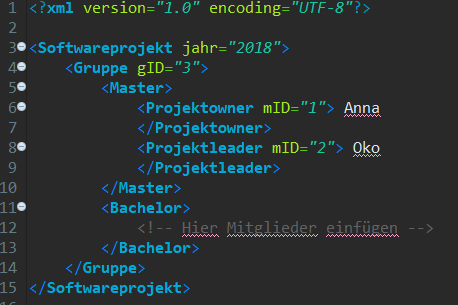
\includegraphics[scale=0.6]{Bilder/XML-Beispiel}
	\caption{Beispielcode XML}
	\label{fig:bild2}
\end{figure}
\nsecend
\nsecbegin{Verwendung}
\begin{itemize}
	\item Erste Zeile im Dokument definiert Version und Codierung
\item Struktur in der Form <tag> ... </tag>, wobei <x> das öffnende Tag und </x> das schließende Tag darstellt
\item Ein Wurzelknoten wird benötigt, der den gesamten XML-Quelltext umfasst
\item Tags sind ineinander geschachtelt
\item Attribute können mit Attribut =''Wert'' im öffnenden Tag definiert werden		
\end{itemize}
\nsecend
\nsecbegin{Bibliotheken in Java}
\begin{itemize}
\item org.xml.sax.* (XML Datei lesen)
\item org.w3c.dom.* (einlesen in den Speicher und schreiben in der Datei)
\item java.xml.parsers.* (Auslesen der XML-Dateien aus dem Speicher und übernehmbar als DOM-Objekt)
\end{itemize}
\nsecend
\nsecend